%%%%%%%%%%%%%%%%%%% EJERCICIO 4 %%%%%%
\textbf{Ejemplo 4}\\
Elaborar una tabla para amortizar la suma de  2.000.000 COP , en las siguientes condiciones:\\
a)	plazo de gracia muerto 6 meses\\
b)	plazo de gracia con cuota reducida al pago de los intereses \\
c)	4 cuotas uniformes a partir del período 4\\
d)	cuota extraordinaria pactada  150.000 COP, en el período 7\\
e)	tasa de interés del 21\% nominal anual trimestre vencido\\


%%%%%%%%%%%%%%%%%%% EJERCICIO 4a-d %%%%%%

%\newpage %USAR SOLO SI EL SOLUCIÓN QUEDA SOLO Y ES NECESARIO BAJARLO A LA SIGUIENTE PAGINA
\textbf{Solución.}\\
%La tabla ira centrada
\begin{center}
	\renewcommand{\arraystretch}{1.5}% Margenes de las celdas
	%Creación de la cuadricula de 3 columnas
	\begin{longtable}[H]{|c|c|c|}
		%Creamos una linea horizontal
		\hline
		%Definimos el color de la primera fila
		\rowcolor[HTML]{FFB183}
		%%%%% INICIO ASIGNACIÓN PERIODO FOCAL %%%%%%%
		%%%%%%%%%% INICIO TITULO
		%Lo que se hace aquí es mezclar las 3 columnas en una sola
		\multicolumn{3}{|c|}{\cellcolor[HTML]{FFB183}\textbf{1. Asignación período focal}}  \\ \hline
		\multicolumn{3}{|c|}{$pf = \textit{0 ptv}$}   \\\hline
		%%%%%%%%%% FIN TITULO
		%%%%% INICIO DECLARACIÓN DE VARIABLES %%%%%%%
		%%%%%%%%%% INICIO TITULO
		%Lo que se hace aquí es mezclar las 3 columnas en una sola
		\multicolumn{3}{|c|}{\cellcolor[HTML]{FFB183}\textbf{2. Declaración de variables}}   \\ \hline
		%%%%%%%%%% FIN TITULO
		%%%%%%%%%% INICIO DE MATEMÁTICAS
		%Cada & hace referencia al paso de la siguiente columna
		\multicolumn{2}{|c|}{$\hspace{2 cm}VP=  2.000.000 \ COP\hspace{2 cm}$} &  \\
		\multicolumn{2}{|c|}{$\hspace{2 cm}j \equiv 21\% \textit{ natv}\hspace{2 cm}$} & $n_0=2 \textit{ ptv}$ \\
		\multicolumn{2}{|c|}{$\hspace{2 cm}i \equiv 5.25\% \textit{ ptv}\hspace{2 cm}$} & $n_1=4 \textit{ ptv}$ \\
		\multicolumn{2}{|c|}{$\hspace{2 cm}F_2= 150.000 \ COP \textit{ natv}\hspace{2 cm}$} & $n_2=7 \textit{ ptv}$ \\
		\multicolumn{2}{|c|}{$\hspace{2 cm}R= COP   \hspace{2 cm}$} &  \\ \hline
		
		
		
		%%%%%%%%%% FIN DE MATEMÁTICAS
		%%%%% FIN DECLARACIÓN DE VARIABLES
		
		
		%%%%% INICIO FLUJO DE CAJA
		\rowcolor[HTML]{FFB183}
		\multicolumn{3}{|c|}{\cellcolor[HTML]{FFB183}\textbf{3. Diagrama de flujo de caja}} \\ \hline
		%Mezclamos 3 columnas y pondremos el dibujo
		%%%%%%%%%%%%% INSERCIÓN DE LA IMAGEN
		%Deberán descargar las imágenes respectivas del drive y pegarlas en la carpeta
		%n_capitulo/img/ejemplos/1/capitulo1ejemplo1.pdf  (el /1/ es el numero del ejemplo)
		\multicolumn{3}{|c|}{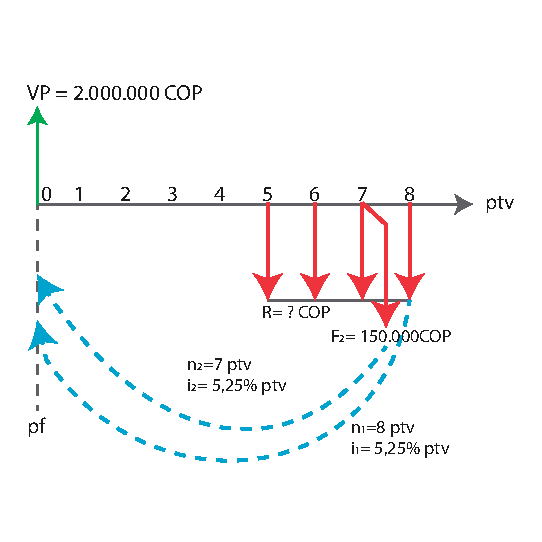
\includegraphics[trim=-78 -5 -78 -5]{7_Capitulo/img/ejemplos/4/Capitulo7Ejercicio4.pdf} }
		
		
		\\ \hline
		%%%%%%%%%%%%% FIN INSERCIÓN DE IMAGEN
		%%%%%FIN FLUJO DE CAJA
		
		
		
		%%%%% INICIO DECLARACIÓN FORMULAS
		%%%%%%%%%%% INICIO TITULO
		\rowcolor[HTML]{FFB183}
		\multicolumn{3}{|c|}{\cellcolor[HTML]{FFB183}\textbf{4. Declaración de fórmulas}}    \\ \hline
		%%%%%%%%%%% FIN TITULO
		%%%%%%%%%%% INICIO MATEMÁTICAS
		\multicolumn{3}{|c|}{$F=P(1+g)^{n} \hspace{0.4 cm} \textit{Valor futuro}$} \\
		\multicolumn{3}{|c|}{$VP=R(\frac{(1-(1+i)^{-n}}{i}) \hspace{0.4 cm} \textit{Valor presente de una serie uniforme vencida}$} \\ \hline
		
		%%%%%%%%%% FIN MATEMÁTICAS
		%%%%%% INICIO DESARROLLO MATEMÁTICO
		\rowcolor[HTML]{FFB183}
		%%%%%%%%%%INICIO TITULO
		\multicolumn{3}{|c|}{\cellcolor[HTML]{FFB183}\textbf{5. Desarrollo matemático}}       \\ \hline
		%%%%%%%%%% FIN TITULO
		%%%%%%%%%% INICIO MATEMÁTICAS
		\multicolumn{3}{|p{\textwidth}|}{Los períodos 1 y 2 son de gracia muertos; los períodos 3 y 4 son de gracia con cuota reducida al valor de los intereses sobre la deuda, capitalizados los intereses en el período de gracias: los periodos 5 al 8 aon sw cuota ordinaria; en el período 2 la deuda sera: } \\
		\multicolumn{3}{|c|}{$F= 2.000.000 \ COP (1+0.0525)^{2}= 2.215.512,50 \ COP $} \\ 
		\multicolumn{3}{|p{\textwidth}|}{El valor del interés I de los períodos 3 y 4, se calcula aplicando la tasa a la deuda que hay en el período 2: } \\ 
		\multicolumn{3}{|c|}{$( 2.215.512,50 \ COP)(0.0525)= 116.314,41 \ COP$} \\
		\multicolumn{3}{|p{\textwidth}|}{La ecuaión de valor quedará así: } \\ 
		\multicolumn{3}{|c|}{$ 2.000.000 \ COP =  116.314,41 \ COP (\frac{(1-(1+0.0525)^{-2}}{0,0525})(1+0.05251)^{-2}+ $} \\
		\multicolumn{3}{|c|}{$+R(\frac{(1-(1+0.0525)^{-4}}{0,0525})(1+0.05251)^{-4}+  150.000 \ COP (1,0525)^{-7}\hspace{0.4 cm} $} \\\hline
		%%%%%%%%%% FIN MATEMÁTICAS
		%%%%%% FIN DESARROLLO MATEMÁTICO
		%%%%%% INICIO RESPUESTA
		\rowcolor[HTML]{FFB183}
		%%%%%%%%%%INICIO TITULO
		\multicolumn{3}{|c|}{\cellcolor[HTML]{FFB183}\textbf{6. Respuesta}}   \\ \hline
		%%%%%%%%%% FIN TITULO
		%%%%%%%%%% INICIO RESPUESTA MATEMÁTICA
		\multicolumn{3}{|c|}{$\mathbf{R= 591.940,10 \ COP}$}
		\begin{comment}
		\multicolumn{3}{|p{\textwidth}|}{
		$F_{4} = F_{5} = 21.609,84 \ COP $ .}
		\end{comment} 
		\\ \hline
		%%%%%%%%%% FIN MATEMÁTICAS
		%%%%%% FIN RESPUESTA
	\end{longtable}
	%Se crean dos lineas en blanco para que no quede el siguiente texto tan pegado
	%\newline \newline %USARLO SI CREES QUE ES NECESARIO
\end{center}
%%%%%%%%%%%%%%%%%%% FIN EJERCICIO 4a-d %%%%%%
%%%%%%%%%%%%%%%%%%% EJERCICIO 4e %%%%%%
\textbf{e.}	Respuesta\\
	La tabla de Amortización será: \\
	\begin{spacing}{1.1}
		\begin{center}
			\begin{tabular}{|p{1cm}|p{2.5cm}|p{2.5cm}|p{2cm}|p{3cm}|}
				\hline
				\textbf{PER\ (1)} & \textbf{SALDO DEUDA (2)=(2)-(5)} & \textbf{INTERESES  (3)=(2)(i)} & \textbf{PAGO\ (4)=R  COP  -  L  COP} & \textbf{AMORTIZACIÓN  (5)=(4)-(3)} \\ \hline
				
				0                 &  2'000.000 COP                      & ---------                       & ---------                       & ---------                          \\ \hline
				1                 &  2'105.000  COP                      &  105.000  COP                   &  0,00  COP                    &    -105.000  COP                    \\ \hline
				2                 &  2'215.512  COP                      &  110.512  COP                   &  0,00  COP                    &    -110.512  COP                   \\ \hline
				3                 &  2'215.512  COP                      &  116.314  COP                  &  116.314  COP                  &    0,00  COP                           \\ \hline
				4                 &  2'215.512  COP                      &  116.314  COP                  &  116.314  COP                  &    0,00  COP                           \\ \hline
				5                 &  1'739.886  COP                       &  116.314  COP                  &  591.940  COP                 &    475.625,59   COP                    \\ \hline
				6                 &  1'239.290  COP                       &  91.344  COP                   &  591.940  COP                 &    500.596  COP                     \\ \hline
				7                 &  562.413  COP                        &   65.062  COP                   &  741.940  COP                 &    676.877   COP                   \\ \hline
				8                 &  0,00  COP                           &  29.526  COP                &    591.940  COP                   &    562.413   COP                    \\ \hline
			\end{tabular}
		\end{center}
	\end{spacing}
	\textbf{Observaciones: }\\
	1)	La amortización de los períodos 1 y 2 es negativa; esto significa que hay una desamortización o aumento de deuda.\\
	2)	La amortización de los períodos 3 y 4 es cero, debido a que se pagan los intereses.\\
	3)	 El valor del pago en el período 7 es igual a la suma del pago ordinario, más el pago extraordinario, por tanto:  591.940,1 
 COP  +  150.000  COP  =  741.940,1  COP.\\
%%%%%%%%%%%%%%%%%%%%%%%%%%FIN EJERCICIO 4e %%%%%%%%%%%%%%%%%%%%%%%%%%%
%%%%%%%%%%%%%%%%%%%%%%%%%%FIN EJERCICIO 4 %%%%%%%%%%%%%%%%%%%%%%%%%%%